%(BEGIN_QUESTION)
% Copyright 2009, Tony R. Kuphaldt, released under the Creative Commons Attribution License (v 1.0)
% This means you may do almost anything with this work of mine, so long as you give me proper credit

Read and outline the ``Sliding-Stem Valves'' section of the ``Control Valves'' chapter in your {\it Lessons In Industrial Instrumentation} textbook.  Note the page numbers where important illustrations, photographs, equations, tables, and other relevant details are found.  Prepare to thoughtfully discuss with your instructor and classmates the concepts and examples explored in this reading.

\underbar{file i04183}
%(END_QUESTION)




%(BEGIN_ANSWER)


%(END_ANSWER)





%(BEGIN_NOTES)

Four types of valve bodies shown: single-ported globe, double-ported globe, gate, and diaphragm.

\vskip 10pt

{\it Direct-acting} valve bodies open up as stem is pulled out of body.  {\it Reverse-acting} valve bodies close down as stem is pushed into body.

\vskip 10pt

STEM-GUIDED GLOBE VALVE: fluid passes through a hole in a ``seat'' which may be covered or plugged by a movable ``plug''.

\vskip 10pt

NEEDLE VALVE: globe design with very small plug.

\vskip 10pt

PORT-GUIDED GLOBE VALVE: plug extends into seat ring for guidance.

\vskip 10pt

DOUBLE-PORTED GLOBE VALVE: two plugs experience opposing forces, less resultant force on stem makes it easier to position.  Difficult to make shut off tightly.  Lapping seats may help, but expansion differences between stem and body will create mis-fit again.

\vskip 10pt

CAGE-GUIDED GLOBE VALVE: piston-shaped plug covers/uncovers holes in cage, throttling flow.

\item{} Unbalanced = higher force from process pressure; easier to tightly shut off
\item{} Balanced = less force from process pressure; harder to tightly shut off
\end{itemize}


\vskip 10pt

MIXING/DIVERTING (3-WAY) GLOBE VALVE: one common port, two complementary ports.  Used for diverting one flow into two, or mixing two flows into one.

\vskip 10pt

GATE VALVE: sliding gate blocks off perpendicular flow.

\vskip 10pt

DIAPHRAGM VALVE: flexible sheet (rubber) pressed against flat surface to shut off.  Useful for slurry flows.  Throttling diaphragm may be directly actuated by air pressure (no separate actuator).

\vskip 10pt








\vskip 20pt \vbox{\hrule \hbox{\strut \vrule{} {\bf Suggestions for Socratic discussion} \vrule} \hrule}

\begin{itemize}
\item{} Explain the operation of stem-guided Masoneilan 21000 valve.
\item{} Describe differences between different types of sliding-stem valves.
\item{} Explain exactly why a double-ported valve has difficulty achieving tight shut-off.
\item{} What is meant by the ``trim'' of a control valve?
\item{} Identify {\it leak paths} past the trim for any of the valve designs shown.  Specifically, where may leakage occur, and how is that leakage mitigated?
\item{} Identify the direction of force applied to the plug of a globe valve by the process fluid's differential pressure.
\end{itemize}









\vfil \eject

\noindent
{\bf Prep Quiz:}

Examples of {\it sliding stem} control valve designs include:

\begin{itemize}
\item{} Disk, plug, and globe
\vskip 5pt 
\item{} Globe, gate, and diaphragm
\vskip 5pt 
\item{} Ball, diaphragm, and globe
\vskip 5pt 
\item{} Butterfly, globe, and ball
\vskip 5pt 
\item{} Disk, ball, and butterfly
\vskip 5pt 
\item{} Globe, disk, and diaphragm
\end{itemize}








\vfil \eject

\noindent
{\bf Prep Quiz:}

{\it Double-ported} globe valves offer both advantages and disadvantages when compared to single-ported globe valves.  Identify one advantage as well as one disadvantage of the double-ported globe valve design over the single-ported globe valve design.

$$\includegraphics[width=15.5cm]{i04183x01.eps}$$








\vfil \eject

\noindent
{\bf Prep Quiz:}

{\it Balanced} cage-guided globe valve trim offer both advantages and disadvantages when compared to {\it unbalanced} cage-guided globe valve trim.  Identify one advantage as well as one disadvantage of the balanced trim design over the unbalanced trim design.



%INDEX% Reading assignment: Lessons In Industrial Instrumentation, Control Valves (sliding-stem control valves)

%(END_NOTES)


